\documentclass[border=10pt,tikz]{standalone}
\usepackage{tikz}
\usetikzlibrary{shapes.geometric, arrows.meta, positioning, calc, fit, backgrounds}
\usepackage{xcolor}
\usepackage{amsmath,amssymb}

% Define Academic Color Palette
\definecolor{tier1border}{HTML}{0284C7}
\definecolor{tier1bg}{HTML}{F0F9FF}
\definecolor{tier1head}{HTML}{E0F2FE}
\definecolor{tier1text}{HTML}{0369A1}

\definecolor{tier2border}{HTML}{059669}
\definecolor{tier2bg}{HTML}{ECFDF5}
\definecolor{tier2head}{HTML}{D1FAE5}
\definecolor{tier2text}{HTML}{065F46}

\definecolor{tier3border}{HTML}{7C3AED}
\definecolor{tier3bg}{HTML}{F5F3FF}
\definecolor{tier3head}{HTML}{EDE9FE}
\definecolor{tier3text}{HTML}{5B21B6}

\definecolor{tier4border}{HTML}{EA580C}
\definecolor{tier4bg}{HTML}{FFF7ED}
\definecolor{tier4head}{HTML}{FFEDD5}
\definecolor{tier4text}{HTML}{9A3412}

\definecolor{tier5border}{HTML}{DC2626}
\definecolor{tier5bg}{HTML}{FEF2F2}
\definecolor{tier5head}{HTML}{FEE2E2}
\definecolor{tier5text}{HTML}{991B1B}

\begin{document}
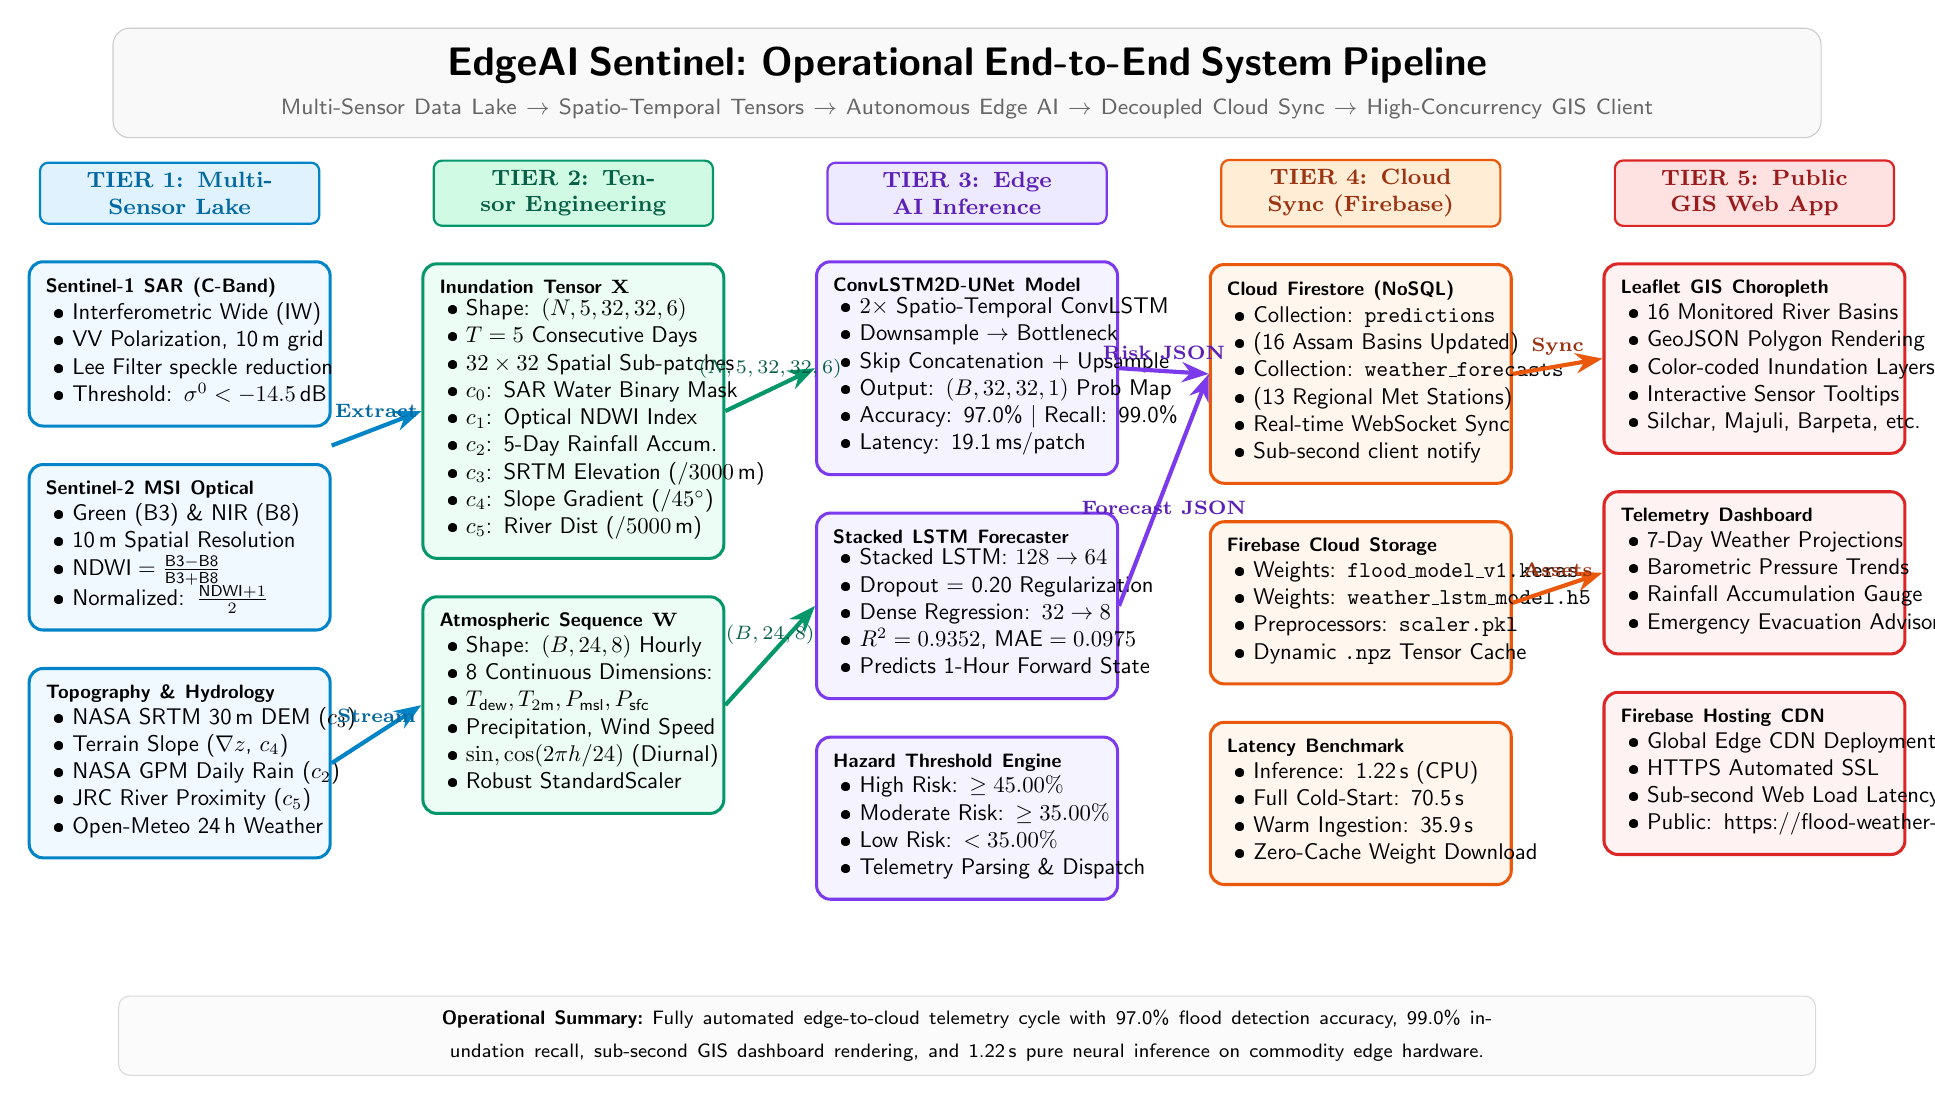
\begin{tikzpicture}[
    font=\sffamily,
    >=Stealth,
    node distance=0.45cm and 0.85cm,
    card/.style={
        rectangle, rounded corners=5pt, line width=1.1pt,
        inner sep=6pt, text width=3.4cm, align=left
    },
    banner/.style={
        rectangle, rounded corners=3pt, line width=0.8pt,
        inner sep=3.5pt, text width=3.3cm, align=center, font=\bfseries\footnotesize
    },
    flow/.style={
        ->, line width=1.5pt, draw=black!70
    },
    subflow/.style={
        ->, line width=1.1pt, draw=black!55, dashed
    }
]

% ==================== TITLE BANNER ====================
\node[draw=gray!40, fill=gray!5, rounded corners=6pt, inner sep=7pt, text width=21.2cm, align=center] (title) at (10.0, 7.6) {
    {\Large\bfseries EdgeAI Sentinel: Operational End-to-End System Pipeline}\\[2pt]
    {\footnotesize\color{gray!80!black}Multi-Sensor Data Lake $\to$ Spatio-Temporal Tensors $\to$ Autonomous Edge AI $\to$ Decoupled Cloud Sync $\to$ High-Concurrency GIS Client}
};

% ==================== TIER 1: DATA LAKE ====================
\node[banner, draw=tier1border, fill=tier1head, text=tier1text] (t1_head) at (0, 6.2) {
    TIER 1: Multi-Sensor Lake
};

\node[card, draw=tier1border, fill=tier1bg, below=of t1_head] (t1_sar) {
    {\bfseries\scriptsize Sentinel-1 SAR (C-Band)}\\
    \scalebox{0.82}{
        \begin{tabular}{@{\textbullet~}l}
        Interferometric Wide (IW)\\
        VV Polarization, 10\,m grid\\
        Lee Filter speckle reduction\\
        Threshold: $\sigma^0 < -14.5$\,dB
        \end{tabular}
    }
};

\node[card, draw=tier1border, fill=tier1bg, below=of t1_sar] (t1_opt) {
    {\bfseries\scriptsize Sentinel-2 MSI Optical}\\
    \scalebox{0.82}{
        \begin{tabular}{@{\textbullet~}l}
        Green (B3) \& NIR (B8)\\
        10\,m Spatial Resolution\\
        $\text{NDWI} = \frac{\text{B3}-\text{B8}}{\text{B3}+\text{B8}}$\\
        Normalized: $\frac{\text{NDWI}+1}{2}$
        \end{tabular}
    }
};

\node[card, draw=tier1border, fill=tier1bg, below=of t1_opt] (t1_hydro) {
    {\bfseries\scriptsize Topography \& Hydrology}\\
    \scalebox{0.82}{
        \begin{tabular}{@{\textbullet~}l}
        NASA SRTM 30\,m DEM ($c_3$)\\
        Terrain Slope ($\nabla z$, $c_4$)\\
        NASA GPM Daily Rain ($c_2$)\\
        JRC River Proximity ($c_5$)\\
        Open-Meteo 24\,h Weather
        \end{tabular}
    }
};

% ==================== TIER 2: TENSOR FORMULATION ====================
\node[banner, draw=tier2border, fill=tier2head, text=tier2text] (t2_head) at (5.0, 6.2) {
    TIER 2: Tensor Engineering
};

\node[card, draw=tier2border, fill=tier2bg, below=of t2_head] (t2_flood) {
    {\bfseries\scriptsize Inundation Tensor $\mathbf{X}$}\\
    \scalebox{0.82}{
        \begin{tabular}{@{\textbullet~}l}
        Shape: $(N, 5, 32, 32, 6)$\\
        $T=5$ Consecutive Days\\
        $32 \times 32$ Spatial Sub-patches\\
        $c_0$: SAR Water Binary Mask\\
        $c_1$: Optical NDWI Index\\
        $c_2$: 5-Day Rainfall Accum.\\
        $c_3$: SRTM Elevation ($/3000\,\text{m}$)\\
        $c_4$: Slope Gradient ($/45^\circ$)\\
        $c_5$: River Dist ($/5000\,\text{m}$)
        \end{tabular}
    }
};

\node[card, draw=tier2border, fill=tier2bg, below=of t2_flood] (t2_weather) {
    {\bfseries\scriptsize Atmospheric Sequence $\mathbf{W}$}\\
    \scalebox{0.82}{
        \begin{tabular}{@{\textbullet~}l}
        Shape: $(B, 24, 8)$ Hourly\\
        8 Continuous Dimensions:\\
        $T_{\text{dew}}, T_{2\text{m}}, P_{\text{msl}}, P_{\text{sfc}}$\\
        Precipitation, Wind Speed\\
        $\sin, \cos(2\pi h / 24)$ (Diurnal)\\
        Robust StandardScaler
        \end{tabular}
    }
};

% ==================== TIER 3: EDGE INFERENCE ====================
\node[banner, draw=tier3border, fill=tier3head, text=tier3text] (t3_head) at (10.0, 6.2) {
    TIER 3: Edge AI Inference
};

\node[card, draw=tier3border, fill=tier3bg, below=of t3_head] (t3_convlstm) {
    {\bfseries\scriptsize ConvLSTM2D-UNet Model}\\
    \scalebox{0.82}{
        \begin{tabular}{@{\textbullet~}l}
        $2\times$ Spatio-Temporal ConvLSTM\\
        Downsample $\to$ Bottleneck\\
        Skip Concatenation + Upsample\\
        Output: $(B, 32, 32, 1)$ Prob Map\\
        Accuracy: 97.0\% $\vert$ Recall: 99.0\%\\
        Latency: 19.1\,ms/patch
        \end{tabular}
    }
};

\node[card, draw=tier3border, fill=tier3bg, below=of t3_convlstm] (t3_lstm) {
    {\bfseries\scriptsize Stacked LSTM Forecaster}\\
    \scalebox{0.82}{
        \begin{tabular}{@{\textbullet~}l}
        Stacked LSTM: $128 \to 64$\\
        Dropout = 0.20 Regularization\\
        Dense Regression: $32 \to 8$\\
        $R^2 = 0.9352$, $\text{MAE} = 0.0975$\\
        Predicts 1-Hour Forward State
        \end{tabular}
    }
};

\node[card, draw=tier3border, fill=tier3bg, below=of t3_lstm] (t3_alert) {
    {\bfseries\scriptsize Hazard Threshold Engine}\\
    \scalebox{0.82}{
        \begin{tabular}{@{\textbullet~}l}
        High Risk: $\ge 45.00\%$\\
        Moderate Risk: $\ge 35.00\%$\\
        Low Risk: $< 35.00\%$\\
        Telemetry Parsing \& Dispatch
        \end{tabular}
    }
};

% ==================== TIER 4: CLOUD SYNC ====================
\node[banner, draw=tier4border, fill=tier4head, text=tier4text] (t4_head) at (15.0, 6.2) {
    TIER 4: Cloud Sync (Firebase)
};

\node[card, draw=tier4border, fill=tier4bg, below=of t4_head] (t4_firestore) {
    {\bfseries\scriptsize Cloud Firestore (NoSQL)}\\
    \scalebox{0.82}{
        \begin{tabular}{@{\textbullet~}l}
        Collection: \texttt{predictions}\\
        (16 Assam Basins Updated)\\
        Collection: \texttt{weather\_forecasts}\\
        (13 Regional Met Stations)\\
        Real-time WebSocket Sync\\
        Sub-second client notify
        \end{tabular}
    }
};

\node[card, draw=tier4border, fill=tier4bg, below=of t4_firestore] (t4_storage) {
    {\bfseries\scriptsize Firebase Cloud Storage}\\
    \scalebox{0.82}{
        \begin{tabular}{@{\textbullet~}l}
        Weights: \texttt{flood\_model\_v1.keras}\\
        Weights: \texttt{weather\_lstm\_model.h5}\\
        Preprocessors: \texttt{scaler.pkl}\\
        Dynamic \texttt{.npz} Tensor Cache
        \end{tabular}
    }
};

\node[card, draw=tier4border, fill=tier4bg, below=of t4_storage] (t4_pipeline) {
    {\bfseries\scriptsize Latency Benchmark}\\
    \scalebox{0.82}{
        \begin{tabular}{@{\textbullet~}l}
        Inference: 1.22\,s (CPU)\\
        Full Cold-Start: 70.5\,s\\
        Warm Ingestion: 35.9\,s\\
        Zero-Cache Weight Download
        \end{tabular}
    }
};

% ==================== TIER 5: CLIENT DELIVERY ====================
\node[banner, draw=tier5border, fill=tier5head, text=tier5text] (t5_head) at (20.0, 6.2) {
    TIER 5: Public GIS Web App
};

\node[card, draw=tier5border, fill=tier5bg, below=of t5_head] (t5_leaflet) {
    {\bfseries\scriptsize Leaflet GIS Choropleth}\\
    \scalebox{0.82}{
        \begin{tabular}{@{\textbullet~}l}
        16 Monitored River Basins\\
        GeoJSON Polygon Rendering\\
        Color-coded Inundation Layers\\
        Interactive Sensor Tooltips\\
        Silchar, Majuli, Barpeta, etc.
        \end{tabular}
    }
};

\node[card, draw=tier5border, fill=tier5bg, below=of t5_leaflet] (t5_dashboard) {
    {\bfseries\scriptsize Telemetry Dashboard}\\
    \scalebox{0.82}{
        \begin{tabular}{@{\textbullet~}l}
        7-Day Weather Projections\\
        Barometric Pressure Trends\\
        Rainfall Accumulation Gauge\\
        Emergency Evacuation Advisory
        \end{tabular}
    }
};

\node[card, draw=tier5border, fill=tier5bg, below=of t5_dashboard] (t5_cdn) {
    {\bfseries\scriptsize Firebase Hosting CDN}\\
    \scalebox{0.82}{
        \begin{tabular}{@{\textbullet~}l}
        Global Edge CDN Deployment\\
        HTTPS Automated SSL\\
        Sub-second Web Load Latency\\
        Public: \url{https://flood-weather-app.web.app}
        \end{tabular}
    }
};

% ==================== INTER-TIER FLOW ARROWS ====================
\draw[flow, draw=tier1border] ($(t1_sar.east)!0.5!(t1_opt.east)$) -- ($(t2_flood.west)!0.5!(t2_flood.west)$)
    node[midway, above, font=\scriptsize\bfseries, color=tier1text] {Extract};

\draw[flow, draw=tier1border] (t1_hydro.east) -- (t2_weather.west)
    node[midway, above, font=\scriptsize\bfseries, color=tier1text] {Stream};

\draw[flow, draw=tier2border] (t2_flood.east) -- (t3_convlstm.west)
    node[midway, above, font=\scriptsize\bfseries, color=tier2text] {$(N,5,32,32,6)$};

\draw[flow, draw=tier2border] (t2_weather.east) -- (t3_lstm.west)
    node[midway, above, font=\scriptsize\bfseries, color=tier2text] {$(B,24,8)$};

\draw[flow, draw=tier3border] (t3_convlstm.east) -- (t4_firestore.west)
    node[midway, above, font=\scriptsize\bfseries, color=tier3text] {Risk JSON};

\draw[flow, draw=tier3border] (t3_lstm.east) -- (t4_firestore.west)
    node[midway, below, font=\scriptsize\bfseries, color=tier3text] {Forecast JSON};

\draw[flow, draw=tier4border] (t4_firestore.east) -- (t5_leaflet.west)
    node[midway, above, font=\scriptsize\bfseries, color=tier4text] {Sync};

\draw[flow, draw=tier4border] (t4_storage.east) -- (t5_dashboard.west)
    node[midway, above, font=\scriptsize\bfseries, color=tier4text] {Assets};

% ==================== FOOTNOTE BANNER ====================
\node[draw=gray!30, fill=gray!3, rounded corners=4pt, inner sep=5pt, text width=21.2cm, align=center] at (10.0, -4.5) {
    {\scriptsize\bfseries Operational Summary:}~{\scriptsize Fully automated edge-to-cloud telemetry cycle with 97.0\% flood detection accuracy, 99.0\% inundation recall, sub-second GIS dashboard rendering, and 1.22\,s pure neural inference on commodity edge hardware.}
};

\end{tikzpicture}
\end{document}
